\chapter{系统设计}
\label{chap:SystemDesign}


\section{系统内核}

\subsection{内核提供的系统调用}
\begin{table}[htb]
    \tableCapSet    % 使用此命令调整 caption 间距
    \caption{tiny 系统调用}
    \label{table:c3tinysyscall}
    \centering
    \zihao{5}
    \begin{tabular}{c|c|c}
        \hlineB{3}  % 线宽为3倍的横线
        编号  & 系统调用               & 功能描述                \\
        \hlineB{2}  % 线宽为2倍的横线
            1&sys\_exit&结束执行 \\
            \hline
            2&sys\_write&输出字符串/写文件 \\
            \hline
            3&sys\_yield&暂时放弃执行 \\
            \hline
            4&sys\_get\_time&获取当前时间 \\
            \hline
            5&sys\_getpid&获取进程id \\
            \hline
            6&sys\_fork&创建子进程 \\
            \hline
            7&sys\_exec&执行新程序 \\
            \hline
            8&sys\_waitpid&等待子进程结束 \\
            \hline
            9&sys\_read&读取字符串/读文件 \\
            \hline
            10&sys\_open&打开/创建文件 \\
            \hline
            11&sys\_close&关闭文件 \\
            \hline
            12&sys\_dup&复制文件描述符 \\
            \hline
            13&sys\_pipe&创建管道 \\
            \hline
            14&sys\_kill&发送信号给某进程 \\
            \hline
            15&sys\_sigaction&设立信号处理例程 \\
            \hline
            16&sys\_sigprocmask&设置要阻止的信号 \\
            \hline
            17&sys\_sigreturn&从信号处理例程返回 \\
            \hline
            18&sys\_sleep&进程休眠一段时间 \\
            \hline
            19&sys\_thread\_create&创建线程 \\
            \hline
            20&sys\_gettid&获取线程id \\
            \hline
            21&sys\_waittid&等待线程结束 \\
            \hline
            22&sys\_mutex\_create&创建锁 \\
            \hline
            23&sys\_mutex\_lock&获取锁 \\
            \hline
            24&sys\_mutex\_unlock&释放锁 \\
            \hline
            25&sys\_semaphore\_create&创建信号量 \\
            \hline
            26&sys\_semaphore\_up&减少信号量的计数 \\
            \hline
            27&sys\_semaphore\_down&增加信号量的计数 \\
            \hline
            28&sys\_condvar\_create&创建条件变量 \\
            \hline
            29&sys\_condvar\_signal&唤醒阻塞在条件变量上的线程 \\
            \hline
            30&sys\_condvar\_wait&阻塞与此条件变量关联的当前线程 \\
        \hlineB{3}
    \end{tabular}
\end{table}

\subsection{内存管理}

从应用程序的视角中,动态内存分配中的内存,依赖于操作系统管理的“堆 (Heap)”。操作系统,需要其能提供动态内存分配。其设计上应当有如下功能:

\begin{itemize}
\item 初始时能提供一块大内存空间作为初始的“堆”。在没有分页机制情况下,这块空间是物理内存空间,否则就是虚拟内存空间。
\item 提供在堆上分配和释放内存的函数接口。这样函数调用方通过分配内存函数接口得到地址连续的空闲内存块进行读写,也能通过释放内存函数接口回收内存,以备后续的内存分配请求。
\item 提供空闲空间管理的连续内存分配算法。相关算法能动态地维护一系列空闲和已分配的内存块,从而有效地管理空闲块。
\item (可选)提供建立在堆上的数据结构和操作。有了上述基本的内存分配与释放函数接口,就可以实现类似动态数组,动态字典等空间灵活可变的堆数据结构,提高编程的灵活性。
\end{itemize}

\subsubsection{GlobalAlloc}
Rust的GlobalAlloc需要在no\_std的环境中提供一个全局的动态内存分配器,Rust将用户提供的分配器来管理堆空间,从而使得与堆相关的智能指针或容器数据结构可以正常工作。具体而言,动态内存分配器需要实现它提供的 Trait约束,具体如下:

\begin{lstlisting}[caption=GlobalAlloc的Trait约束]
pub unsafe fn alloc(&self, layout: Layout) -> *mut u8;
pub unsafe fn dealloc(&self, layout: Layout);
\end{lstlisting}

当完成Heap的接入的时候,在no\_std的环境中任然还需要为其提供, 当动态内存分配失败时,系统的处理函数, 简单处理,让\verb|#[alloc_error_handler]|直接返回\verb|panic|的异常。

\subsubsection{地址空间}

地址空间,从某种程度上讲,可以将它看成一块巨大但并不一定真实存在的内存。在每个应用程序的视角里,操作系统分配给应用程序一个地址范围受限(容量很大),独占的连续地址空间(其中有些地方被操作系统限制不能访问,如内核本身占用的虚地址空间等),因此应用程序可以在划分给它的地址空间中随意规划内存布局,它的各个段也就可以分别放置在地址空间中它希望的位置(当然是操作系统允许应用访问的地址)。应用同样可以使用一个地址作为索引来读写自己地址空间的数据,就像用物理地址作为索引来读写物理内存上的数据一样。这种地址被称为 虚拟地址 (Virtual Address) 。


\subsubsection{分页管理}

具体的分页逻辑参考\autoref{figure:c2addressv2p}, 其思路来自Riscv平台下的Sv39的地址转换。

内核以页为单位进行物理内存管理。每个应用的地址空间可以被分成若干个(虚拟) 页面 (Page) ,而可用的物理内存也同样可以被分成若干个(物理) 页帧 (Frame) ,虚拟页面和物理页帧的大小相同。每个虚拟页面中的数据实际上都存储在某个物理页帧上。

为了方便实现虚拟页面到物理页帧的地址转换,标记每个虚拟页面和物理页帧一个编号,分别称为 虚拟页号 (VPN, Virtual Page Number) 和 物理页号 (PPN, Physical Page Number) 。每个应用都有一个表示地址映射关系的 页表 (Page Table) ,里面记录了该应用地址空间中的每个虚拟页面映射到物理内存中的哪个物理页帧,即数据实际被内核放在哪里。

如果将页表看成一个键值对,其键的类型为虚拟页号,值的类型则为物理页号。当 MMU 进行地址转换的时候,虚拟地址会分为两部分(虚拟页号,页内偏移),MMU首先找到虚拟地址所在虚拟页面的页号,然后查当前应用的页表,根据虚拟页号找到物理页号;最后按照虚拟地址的页内偏移,给物理页号对应的物理页帧的起始地址加上一个偏移量,这就得到了实际访问的物理地址。

\subsubsection{内核与应用地址的空间分配}

在分页模式开启之后,CPU先拿到虚存地址,需要通过 MMU 的地址转换变成物理地址,再交给 CPU 的访存单元去访问物理内存。地址空间抽象的重要意义在于 隔离 (Isolation) ,当内核让应用执行前,内核需要控制 MMU 使用这个应用的多级页表进行地址转换。由于每个应用地址空间在创建的时候也顺带设置好了多级页表,使得只有那些存放了它的代码和数据的物理页帧能够通过该多级页表被映射到,这样它就只能访问自己的代码和数据而无法触及其他应用或内核的内容。

启用分页模式下,内核代码的访存地址也会被视为一个虚拟地址并需要经过 MMU 的地址转换,因此也需要为内核构造一个地址空间,它除了允许内核的各数据段能够被正常访问之后,还应包含所有应用的内核栈以及一个跳板 (Trampoline) 。

通常在内核空间中跳板放在最高的一个虚拟页面中,因为分页机制的关系,使得每次发生Trap的时候,Riscv的satp的会发生改变,而trap的异常处理函数只有在内核空间中才能被访问,因此如此设计可以设计在地址空间切换时指令能够被正确执行。接下来则是从高到低放置每个应用的内核栈。

应用空间,效仿内核地址空间的设计,同样借助页表机制使得应用地址空间的各个逻辑段也可以有不同的访问方式限制,这样可以提早检测出应用的错误并及时将其终止以最小化它对系统带来的恶劣影响。

\subsubsection{Yield系统调用}

需要知道当前所处的地址空间,用户的上下文,还要相应的地址映射关系。由于内核空间和用户空间之间的转换是通过跳板页实现的,因此用户的上下文,将会被存放在跳板也的数据段中,而在分页机制的情况下,相应上下文的地址可以通过相应的公式计算出来(用户可以获取一页的空间保存上下文)。

参考tornado-os的设计,利用tp寄存器,由其指向一个存有KernelHartInfo的地址。而用户的地址空间映射就被包存在这里。

\begin{lstlisting}[caption=KernelHartInfo的结构]
#[repr(C)]
pub struct KernelHartInfo {
    hart_id: usize,
    // ...
    asid_alloc: (LinkedList<usize>, usize),   // (空余的编号回收池,目前已分配最大的编号)
    user_mm_sets: (LinkedList<MemorySet>, usize), // (注册的用户地址空间映射,上一次进入的用户地址空间编号)
}
\end{lstlisting}

KernelHartInfo游走在内核态和用户态之间。记录了如CPU的核心编号, 用户空间的地址映射信息,地址分配的信息等等。

\subsection{进程通信}

为了在用户态就可以借助操作系统的服务动态灵活地管理和控制应用的执行,我们需要在已有的 任务 抽象的基础上进一步扩展,形成新的抽象: 进程 ,并实现若干基于 进程 的强大系统调用。

\begin{itemize}
\item 创建 (Create):父进程创建新的子进程。用户在 shell 中键入命令或用鼠标双击应用程序图标(这需要 GUI 界面,目前我们还没有实现)时,会调用操作系统服务来创建新进程,运行指定的程序。
\item 销毁 (Destroy):进程退出。进程会在运行完成后可自行退出,但还需要其他进程(如创建这些进程的父进程)来回收这些进程最后的资源,并销毁这些进程。
\item 等待 (Wait):父进程等待子进程退出。父进程等待子进程停止是很有用的,比如上面提到的收集子进程的退出信息,回收退出的子进程占用的剩余资源等。
\item 信息 (Info):获取进程的状态信息:操作系统也可提供有关进程的身份和状态等进程信息,例如进程的ID,进程的运行状态,进程的优先级等。
\item 其他 (Other):其他的进程控制服务。例如,让一个进程能够杀死另外一个进程,暂停进程(停止运行一段时间),恢复进程(继续运行)等。
\end{itemize}

参照rcore的设计, 进程模型有三个运行状态:就绪态、运行态和等待态;有基于独立页表的地址空间;可被操作系统调度来分时占用 CPU 执行;可以动态创建和退出;可通过系统调用获得操作系统的服务。与之对应的一些重要的结构。

\begin{itemize}
\item 进程标识符 PidHandle 以及内核栈 KernelStack :进程控制块的重要组成部分。
\item 任务控制块 TaskControlBlock :表示进程的核心数据结构。
\item 任务管理器 TaskManager :管理进程集合的核心数据结构。
\item 处理器管理结构 Processor :用于进程调度,维护进程的处理器状态。
\end{itemize}

从而与之对应的重要的功能

\begin{itemize}
\item 创建初始进程:创建第一个用户态进程 initproc;
\item 进程调度机制:当进程主动调用 sys\_yield 交出 CPU 使用权或者内核把本轮分配的时间片用尽的进程换出且换入下一个进程;
\item 进程生成机制:两个重要系统调用 sys\_fork/sys\_exec 的实现;
\item 进程资源回收机制:当进程调用 sys\_exit 正常退出或者出错被内核终止之后如何保存其退出码,其父进程通过 sys\_waitpid 系统调用收集该进程的信息并回收其资源。
\item 字符输入机制:为了支持shell程序user\_shell获得字符输入,介绍 sys\_read 系统调用的实现;
\end{itemize}

内核初始化完毕之后会调用由 task 子模块提供的 add\_initproc 函数将初始进程加入任务管理器。通过task模块提供的suspend\_current\_and\_run\_next函数可以暂停当前任务并切换到下一个任务,此时会调用sys\_yield主动交出使用权、本轮时间片用尽或者由于某些原因内核中的处理无法继续的时候,就会在内核中调用此函数触发调度机制并进行任务切换。

在内核中手动生成的进程只有初始进程 initproc ,余下所有的进程都是它直接或间接 fork 出来的。当一个子进程被 fork 出来之后,它可以调用 exec 系统调用来加载并执行另一个可执行文件。因此, fork/exec 两个系统调用提供了进程的生成机制。

在子进程内核栈上压入一个初始化的任务上下文,使得内核一旦通过任务切换到该进程,就会跳转进入用户态。而在复制地址空间的时候,子进程的 Trap 上下文也是完全从父进程复制过来的,这可以保证子进程进入用户态和其父进程回到用户态的那一瞬间 CPU 的状态是完全相同的(后面我们会让它们的返回值不同从而区分两个进程)。而两个进程的应用数据由于地址空间复制的原因也是完全相同的。

sys\_waitpid 是一个立即返回的系统调用,它的返回值语义是:如果当前的进程不存在一个进程 ID 为 pid(pid==-1 或 pid > 0)的子进程,则返回 -1;如果存在一个进程 ID 为 pid 的僵尸子进程,则正常回收并返回子进程的 pid,并更新系统调用的退出码参数为 exit\_code 。这里还有一个 -2 的返回值,它的含义是子进程还没退出,通知用户库 user\_lib (是实际发出系统调用的地方),这样用户库看到是 -2 后,就进一步调用 sys\_yield 系统调用,让当前父进程进入等待状态。

\subsubsection{管道}


管道是一种进程间通信机制,由操作系统提供,并可通过直接编程或在shell程序的帮助下轻松地把不同进程(目前是父子进程之间或子子进程之间)的输入和输出对接起来。也可以将管道看成一个有一定缓冲区大小的字节队列,它分为读和写两端,需要通过不同的文件描述符来访问。读端只能用来从管道中读取,而写端只能用来将数据写入管道。由于管道是一个队列,读取数据的时候会从队头读取并弹出数据,而写入数据的时候则会把数据写入到队列的队尾。由于管道的缓冲区大小是有限的,一旦整个缓冲区都被填满就不能再继续写入,就需要等到读端读取并从队列中弹出一些数据之后才能继续写入。当缓冲区为空的时候,读端自然也不能继续从里面读取数据,需要等到写端写入了一些数据之后才能继续读取。

\subsubsection{信号}

信号(Signals)是类 UNIX 操作系统中实现进程间通信的一种异步通知机制,用来提醒某进程一个特定事件已经发生,需要及时处理。当一个信号发送给一个进程时,操作系统会中断接收到信号的进程的正常执行流程并对信号进行处理。如果该进程定义了信号的处理函数,那么这个处理函数会被调用,否则就执行默认的处理行为,比如让该进程退出。在处理完信号之后,如果进程还没有退出,则会恢复并继续进程的正常执行。

\subsection{文件系统}


\subsubsection{文件}

在操作系统的用户看来,常规文件是保存在持久存储设备上的一个字节序列,每个常规文件都有一个 文件名 (Filename) ,用户需要通过它来区分不同的常规文件。方便起见,在下面的描述中,“文件”有可能指的是常规文件、目录,也可能是之前提到的若干种进程可以读写的 标准输出、标准输入、管道等I/O 资源,请同学自行根据上下文判断取哪种含义。

\subsubsection{目录}

早期的文件系统通过文件名来区分文件,但是这会造成一些归档和管理上的困难。如今的使用习惯是将文件根据功能、属性的不同分类归档到不同层级的目录之下。这样就很容易逐级找到想要的文件。结合用户和用户组的概念,目录的存在也使得文件访问权限控制更加容易,只需要对于目录进行设置就可以间接设置用户/用户组对该目录下所有文件的访问权限,这使得操作系统能够更加安全的支持多用户情况下对不同文件的访问。

\subsubsection{文件的读写和权限结构}

\begin{lstlisting}[caption=文件系统基本读写]
pub trait File: Send + Sync {
    fn readable(&self) -> bool;
    fn writable(&self) -> bool;
    fn read(&self, buf: UserBuffer) -> usize;
    fn write(&self, buf: UserBuffer) -> usize;
}
\end{lstlisting}

\begin{itemize}
\item r 表示是否允许获取该目录下有哪些文件和子目录;
\item w 表示是否允许在该目录下创建/删除文件和子目录;
\item x 表示是否允许“通过”该目录。
\end{itemize}


\subsubsection{Easy-fs\pagescite{rcore0}的磁盘布局}

\begin{figure}[htb]
    \figureCapSet
    \centering
    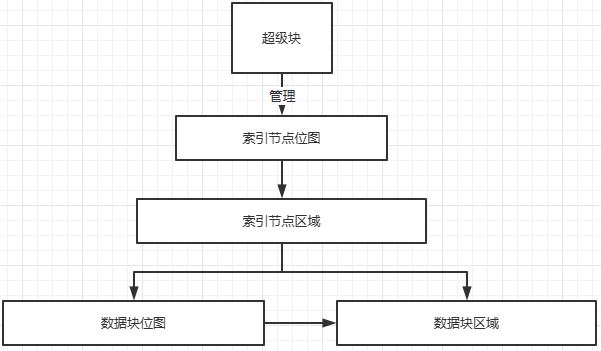
\includegraphics[width=.8\linewidth]{figure/c3/easyfsdevicemap.png}
    \caption{Easy Fs 的磁盘布局}
    \label{figure:c3easyfsdevicemap}
\end{figure}


最开始的区域的长度为一个块,其内容是 easy-fs 超级块 (Super Block)。超级块内以魔数的形式提供了文件系统合法性检查功能,同时还可以定位其他连续区域的位置。

第二个区域是一个索引节点位图,长度为若干个块。它记录了后面的索引节点区域中有哪些索引节点已经被分配出去使用了,而哪些还尚未被分配出去。

第三个区域是索引节点区域,长度为若干个块。其中的每个块都存储了若干个索引节点。

第四个区域是一个数据块位图,长度为若干个块。它记录了后面的数据块区域中有哪些数据块已经被分配出去使用了,而哪些还尚未被分配出去。

最后的区域则是数据块区域,顾名思义,其中的每一个已经分配出去的块保存了文件或目录中的具体数据内容。


\subsection{并发处理}

线程是进程的组成部分,进程可包含1 – n个线程,属于同一个进程的线程共享进程的资源,比如地址空间,打开的文件等。线程基本上由线程ID、执行状态、当前指令指针(PC)、寄存器集合和栈组成。线程是可以被操作系统或用户态调度器独立调度(Scheduling)和分派(Dispatch)的基本单位。

进程是程序的基本执行实体,是程序对某数据集合进行操作的一次执行过程,是系统进行资源(处理器,地址空间和文件等)分配和调度的基本单位。在有了线程后,对进程的定义也要调整了,进程是线程的资源容器,线程是程序的基本执行实体。

数据不一致性、不确定的计算结果,意味在操作系统的执行过程中,可能存在并发问题,并导致程序或操作系统执行失败。我们先给出 线程的数据一致性 的定义:在单处理器(即只有一个核的CPU)下,如果某线程更新了一个可被其他线程读到的共享数据,那么后续其他线程都能读到这个最新被更新的共享数据。当多个线程共享同一进程的地址空间时,每个线程都可以访问属于这个进程的数据(全局变量)。如果每个线程使用到的变量都是其他线程不会读取或者修改的话,各个线程访问的变量与预期结果一样,那么就不存在一致性问题。如果变量是只读的,多个线程读取该变量与预期结果一致,也不会有一致性问题。

当两个或多个线程在竞争访问同一资源时,执行结果取决于它们的不可预知的执行顺序的情况称为 线程的竞态条件。竞态条件是一种常见的并发问题,可能导致应用程序或操作系统执行失败。而线程的数据不一致问题和竞态条件问题的根本原因是调度的不可控性 :即读写共享变量的代码片段会随时可能被操作系统调度和切换。

\subsubsection{互斥锁}

互斥锁是操作系统中用于保护共享资源的机制。互斥锁能够确保在任何时候只有一个线程访问共享资源,从而避免资源竞争导致的数据不一致的问题。在获取互斥锁的时候,线程会被挂起,直到另一个线程释放了锁。

\subsubsection{条件变量}

条件变量是操作系统中的一种同步原语,可用于在多个线程之间进行协作,即允许一个线程在另一个线程完成某些操作之前等待。条件变量与互斥锁经常一起使用,以保证在同一时刻只有一个线程在访问共享资源。

线程通过更改布尔值并通知条件变量来发送信号,而主线程则使用条件变量来等待信号。首先,定义一个元组 (Mutex<bool>, Condvar),并使用 Arc(原子引用计数)将其包装在一个可共享的指针中。这个指针有两个副本,因此两个线程都可以访问这个元组。然后,启动一个新的线程,并在这个线程内部使用互斥锁来更改共享的布尔值。最后,它使用条件变量来等待这个布尔值被更改,最后退出循环。

\subsubsection{信号量}

信号量是操作系统中的一种同步原语,用于在多个线程或进程之间共享资源时进行互斥访问。它通常是一个整数值,用于计数指定数量的资源可用。当一个线程需要使用资源时,它会执行信号量的获取操作,如果信号量的值小于等于零,则线程将被挂起,(直到信号量的值变为正数,则会被唤醒);否则将信号量的值减一,操作正常返回。另一方面,当一个线程完成使用资源后,它可以执行信号量的释放操作,将信号量的值加一,并唤醒一个或所有挂起的线程。

\section{异步调度}

\subsection{ring\_scheduler}


ring\_scheduler中的黑盒调度任务池资源,同时为内核和用户提供一系列的数据接口,实现任务资源在内核态和用户态两者之间的统一调度。

\subsubsection{元数据}

元数据是ring\_scheduler基本的调度单位

\begin{itemize}
\item hart\_id: 运行该任务的硬件线程编号,简单化为核的ID号
\item address\_space\_id: 地址空间编号
\item task\_repr: 任务指针,由所在的地址空间解释为任务
\item state: 任务状态
\end{itemize}


address\_space\_id指示任务地址,在分页机制下,通过KernelHartInfo,取得地址空间的映射关系,找到任务执行的物理地址。

task\_repr是任务指针,内核空间和用户空间的任务在ring\_scheduler由其指代,同时只有当task\_repr通过正确的地址转换才能得到正确的任务结构。

如果task\_repr在其他地址空间尝试被解释,那么很可能会触发缺页异常,就算可以被转换,转换出来的数据也是不对的。这得益于指令集设计上的地址空间隔离的作用,可以实现一定的安全性保障。


state标记这个任务的状态,至少会有两种状态的存在:就绪与睡眠。就绪状态的任务表示该任务的某个阶段已经准备好可以进一步执行;睡眠状态的任务表示该任务需要等待一些数据或者其他任务的完成,处于等待状态。

就绪状态的任务可以被ring\_scheduler弹出交给内核或用户运行,睡眠状态的任务只有被唤醒器唤醒之后才能转成就绪状态,然后被进一步执行。

\subsubsection{ring\_scheduler的接口}

\begin{lstlisting}[caption=调度器的接口约束]
pub trait Scheduler<T: Clone + PartialEq> {
    type Priority;
    fn add_task(&mut self, task: T) -> Option<T>;
    fn peek_next_task(&self) -> Option<&T>;
    fn peek_next_task_mut(&mut self) -> Option<&mut T>;
    fn next_task(&mut self) -> Option<T>;
    fn current_task(&self) -> Option<T>;
    fn remove_task(&mut self, task: &T);
    fn set_priority(&mut self, task: T, priority: Self::Priority);
    fn queue_len(&self) -> Option<usize> {
        None
    }
}
\end{lstlisting}


\begin{itemize}
\item add\_task:尝试向调度器中添加一个任务
\item peek\_next\_task:获取下一个任务不可变的引用
\item peek\_next\_task\_mut:获取下一个任务可变的引用
\item next\_task: 得到下一个任务
\item current\_task:获取正在运行的当前任务,在发生中断时,通过这个保存任务的上下文
\item remove\_task:从调度器中移除一个任务
\item set\_priority: 设置任务的优先级,没有实现
\item queue\_len:返回队列的长度,如果不存在,则返回None
\end{itemize}


\subsubsection{先来先服务的队列处理方式}

这里采用最简单的任务调度算法,ring\_scheduler的底层实现了一个循环队列用以存储相应的任务结构,和相应的一些操作。底层队列的长度将是固定的,当队列中的任务处于唤醒时或队列已经放不下相应任务时,ring\_scheduler会将相应任务弹出,对于后者则阻止新任务的队列加入。

\subsection{异步}

调度器和执行器是分离的。调度器只根据元数据调度,得到下一个任务是什么。而这个任务该如何运行,调度器不知道,需要交给执行器来解释元数据的意义,拿到异步结构之后运行。

\subsubsection{任务的状态}

\begin{equation}
    \label{equation:c3taskstate}
    \begin{aligned}
\boldsymbol{\mathrm{TaskState}} = (\mathrm{Ready}, \mathrm{Sleeping}, \mathrm{Finished})^{\mathrm{T}}
    \end{aligned}
\end{equation}

其中,任务有TaskRepr的指针传递进来, 其中如果状态为Ready时, 表示任务可以执行,应当被ring\_scheduler弹出。Sleeping则表示任务处于休眠状态, 当ring\_scheduler中的任务睡眠的程度到达内核约束的值或,应当由内核通过一定方式尝试唤醒适量的任务。最后, Finished则表示任务已经完成。

\subsubsection{共享的数据}

参考元数据, $\boldsymbol{\mathrm{Task}} := (\mathrm{hartId}, \mathrm{addressSpaceId}, \mathrm{taskRepr}, \mathrm{State})^{\mathrm{T}}$。为了使得内核和用户态的任务可以得到共享,因此内核态和用户态的任务都应当有如下描述:

\begin{lstlisting}
struct Task {
    pub id: TaskId,
    pub process: Arc<Process>,
    pub inner: Mutex<TaskInner>,
    pub future: Mutex<Pin<Box<dyn Future<Output = ()> + 'static + Send + Sync>>>, 
}
\end{lstlisting}

\subsubsection{执行器的实现}

由于调度器和执行器是分离的,调度器只知道任务的运行状态,而不知道该如何对任务进行操作。因此后半部分的工作将需要执行器的介入,而执行器的工作依赖于调度器的返回,若执行器返回遵循以下的规则

\begin{equation}
    \label{equation:c3schedulerreturn}
    \begin{aligned}
\boldsymbol{\mathrm{SchedulerReturn}} = (\mathrm{TaskRepr}, \mathrm{SholdYield}, \mathrm{NoWakeTask}, \mathrm{Finished})^{\mathrm{T}}
    \end{aligned}
\end{equation}

其中

\begin{itemize}
    \item TaskRepr, 应当立即执行特定任务, 执行器从调度器获得这个值的时候需要调用相关方法释放任务,如果不释放任务,再次执行,还是会得到相同的任务。
    \item ShouldYield, 其他地址空间的任务要运行,应当提示执行器主动让出,并携带下一个地址空间信息。这时候在用户态应该执行yield系统调用,yield系统调用将保存当前用户上下文,陷入内核并切换到下一个地址空间去运行。
    \item  NoWakeTask,调度器里面没有醒着的任务,但存在睡眠的任务。
    \item  Finished,队列已空,所有任务已经结束。
\end{itemize}


内核执行器的设计

在一个大循环中,不断从共享调度器中拿到任务,对任务进行poll操作,如果返回Ready,从共享调度器中删除该任务,如果返回Pending,将该任务设置为睡眠状态。如果共享调度器中所有任务都已完成,则退出系统。

\begin{lstlisting}[caption=内核执行器的设计]
pub fn run_until_idle() {
    loop {
        let task = peek_task(); // 从共享调度器中拿出下一个任务的指针,不弹出
        match task {
            TaskResult::Task(task_repr: usize) => { // 任务指针
                set_task_state(task_repr, TaskState::Sleeping); // 设置任务的状态为睡眠
                let task: Arc<KernelTask> = unsafe { Arc::from_raw(task_repr as *mut _) };
                // 注册 waker
                let waker = waker_ref(&task);
                let mut context = Context::from_waker(&*waker);
                let ret = task.future.lock().as_mut().poll(&mut context);
                if let Poll::Pending = ret {
                    core::mem::forget(task); // 不要释放task的内存,它将继续保存在内存中被使用
                } else {
                    // 否则,从共享调度器中删除此任务
                    delete_task(task_repr);
                } // 隐含一个drop(task)
            },
            TaskResult::ShouldYield(next_asid: usize) => {...}, // 不同地址空间的任务,需要切换地址空间
            TaskResult::NoWakeTask => {...},
            TaskResult::Finished => {...}
        }
    }
}
\end{lstlisting}

用户执行器的设计

用户执行器的设计和内核执行器存在一点区别,就是当拿到不在当前地址空间的任务的时候,不释放这个任务的内存,执行切换地址空间的系统调用。

\begin{lstlisting}[caption=用户执行器的设计]
pub fn run_until_idle() {
    loop {
        let task = peek_task(); // 从共享调度器中拿出下一个任务的指针,不弹出
        match task {
            TaskResult::Task(task_repr: usize) => {...},
            TaskResult::ShouldYield(next_asid: usize) => {
                mem::forget(task);
                do_yield(next_asid);
            },
            TaskResult::NoWakeTask => {...},
            TaskResult::Finished => {...}
        }
    }
}
\end{lstlisting}

\section{模块设计}

\subsection{静态模块}

在静态模块的设计中,系统模块设计应当遵循以下原则:

\begin{enumerate}
    \item 最小正交化的模块
    \item 树状依赖和空间隔离
\end{enumerate}

\subsubsection{最小正交的模块}


\begin{figure}[htb]
    \figureCapSet
    \centering
    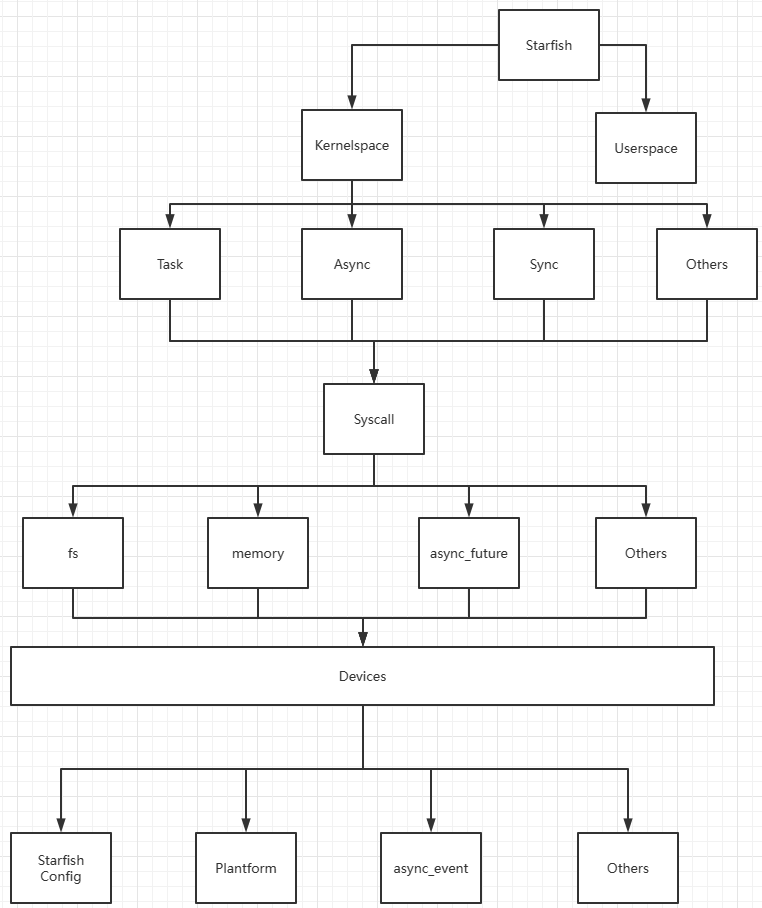
\includegraphics[width=.8\linewidth]{figure/c3/starfishstructure.png}
    \caption{Starfish 的静态模块分解图}
    \label{figure:c3starfishstructure}
\end{figure}

参考\autoref{figure:c3starfishstructure},这是最开始设计的内核模块的静态的拆分图。为了方便描述,每一层定义为抽象层级,处在最底层的其抽象层级为0,层级越低抽象的能力越小,反之则越大。而每一层的节点可以定义为抽象因子。例如,Starfish Config为0层的抽象因子,其寓意为在该层级的最小正交因子(即在当前的抽象下,该因子为最小的不可再分割的正交参考)。

正交,顾名思义就是将一个复杂的“合力”,通过相应的参考系,进行有序分解,形成一个可以通过参考系中的相应因子描述的矢量,例如 $\boldsymbol {v}=(a, b)$, 则可以准确表述矢量$\boldsymbol {v}$在直角坐标系中的空间表示。

类比前者,提出抽象正交化的概念,我们将整个抽象空间则概括为由抽象层级和抽象因子组成的抽象评估空间,其空间的单位为抽象评估因子,则可以得到如下式子,


\begin{equation}
    \label{equation:c3elf}
    \begin{aligned}
       \boldsymbol{\mathrm{E}} = (L, F)
    \end{aligned}
\end{equation}

其中$\boldsymbol{E}$表示评估因子,L表示抽象层级,F表示抽象因子。由此可以总结出两组概念:最小正交化和严格最小正交化。

\begin{enumerate}
    \item 最小正交化: 当$L=0$时,即抽象层级为0,即模块不可再分的情况下, $\boldsymbol{E}$为最小正交化的评估因子,此时模块分解为最小正交化。
    \item 严格最小正交化: 在满足最小正交化的前提下, 有$F = {F_{0}, F_{1}, \cdots, F_{n}}$,其中$0 = {F_{0} \cap F_{1} \cap \cdots \cap F_{n}}$, 此时, $\boldsymbol{E}$为严格正交化的评估因子,此时模块分解为严格最小正交化。
\end{enumerate}

当$\boldsymbol{E}$为严格正交化时,则可以说模块分解达到了一个最优的状态,此时所有的$L=0$级的模块之间不存在互相干扰的情况,彼此之间的联系,仅仅通过语言编程者之间的API约束,如此的好处可以使得模块之间的耦合程度变低,相互之间可以独立进行开发,同时如果他人的内核也遵循了相应的API约束,则该模块可以达到共享的目的。


\subsubsection{树状依赖和空间隔离}


通过\autoref{figure:c3starfishstructure}的观察,可以发现模块的分解和组合,其静态的模块将会形成一种树状的结果,此时L(即抽象层级)之间是存在“方向”的,即当存在$L_{i} < L_{j} (i < j)$时, $L_{j}$必然是由部分$L_{i}$组成,而必不可能存在上下互换的生成形式,如若L的层级方向出现错误,则$\boldsymbol{E}$将无法做出评估,其模块拆解也必然是错误的。由此,一个良好的模块分解必然会形成一个层次分明的树状依赖。

当L一定, $F = {F_{0}, F_{1}, \cdots, F_{n}}$时, 若有$0 = {F_{0} \cap F_{1} \cap \cdots \cap F_{n}}$,此时的$\boldsymbol{E}$可以达到最优解,即优化评估因子,记作$\boldsymbol{OE}$,特别地当 $L = 0$时,若形成$\boldsymbol{OE}$,即$F$达到分解地最优解,则此时就可以称为严格最小正交化。

其中$\boldsymbol{OE}$的意义是,层级间的依赖被解除,模块是独立,没有相互干扰, 可以达到层级空间间的空间隔离。同样以此可以逆向评估底层模块的$\boldsymbol{E}$特性, 通过数学归纳法,我们可以显而易见的得出当$L_{i} < L_{j} (i < j)$, 若$L_{j}$达到了$\boldsymbol{OE}$,则$L_{i}$也应当是$\boldsymbol{OE}$的。

\subsection{动态模块}

在动态模块的设计中,系统的模块设计应当遵循以下三个原则: \begin{enumerate}
    \item 需要获取所有模块的运行时的持久边界
    \item 最大限度地发挥语言(Rust)和编译器的作用
    \item 最小化模块之间的状态溢出
\end{enumerate}

\subsubsection{需要获取所有模块的运行时的持久边界}

系统内核中的模块组件具有明确定义的边界(严格化的正交模块),并在整个运行时保持不变: 在实现时,系统模块组件以Rust独立的Crate的形式存在;在编译时,系统模块组件以一组加载的内存区域的形式存在;在运行时,系统模块组件以一组加载内存区域的形式存在,内存区域具有每部分的边界和依赖元数据。

上述的设计原则每一个内核的系统模块组件都需要遵循。运行时,可以显示识别系统模块组件的边界是系统内核中组件隔离和状态管理的基础。

在运行时,系统内核根据需要将所有系统模块组件加载并链接到系统中。简而言之,这需要找到并解析系统模块组件对象,将其部分加载到内存中,解析其依赖,根据依赖树,以写入连接器重定位条目,根据需要递归加载任何丢失的系统模块组件,并向符号映射添加新的公共符号。基于此可以为内核进化和故障恢复提供理论基础。加载的系统模块组件集定义了一个系统模块组件空间,一个包含所有系统模块组件公共符号的真正的名称空间,用于快速解析单元格之间的依赖关系。每个加载的系统模块组件节点跟踪其组成部分和存储区域包含它们。每个系统模块组件中的部分对应于其Crate的目标文件中的部分,例如,可执行文件、只读数据和读写数据部分。每个加载的分段节点跟踪其大小、在存储器中的位置以及双向依赖性(输入和输出);额外的元数据用于加速系统模块组件交换和其他系统功能。

系统模块组件边界的持久性降低了复杂性: 系统内核的持久性系统模块组件边界在其存在的所有阶段提供了一致的系统结构抽象。这将会降低了开发者对系统的理想模型的复杂性,并简化了故障恢复和演化逻辑,因为系统内核可以在运行时从相同的面向系统模块组件的角度自省和管理它自己的代码。从顶层应用程序和库到核心内核组件的一切都可以作为系统模块组件来观察。这使得系统内核能够

\begin{itemize}
	\item 实现统一适用于任何单元的单一机制,即模块交换,以及
	\item 以安全的方式从多个系统层(例如,应用和内核组件)联合进化模块。
\end{itemize}

\subsubsection{最大限度地发挥语言(Rust)和编译器的作用}
通过使编译器能够最大限度地检查安全性和正确性不变量来最大限度发挥语言的力量。

将系统内核的执行环境与该语言的运行时模型相匹配,并在Rust等现代语言提供的强大的静态类型系统中实现操作系统概念。这将编译器检查的不变量(例如,没有悬空引用)扩展到了所有类型的资源,而不仅仅是语言中内置的那些。

依赖语言设计有两个主要好处:

\begin{itemize}
    \item 首先,它使编译器能够接管资源管理职责,减少了操作系统必须维护的状态,从而减少了状态溢出并加强了隔离。
    \item 它使编译器能够在理解代码行为的过程中应用安全检查,从应用程序到核心内核组件实现端到端安全,并将语义运行时错误转化为编译时错误。
\end{itemize}

相比之下,传统的非语言方法依赖于硬件保护和运行时检查来维护安全性、隔离性和正确性的不变量。这些特性对编译器是透明的,需要不安全的代码。甚至现有的安全语言操作系统。在语言级别的安全代码和底层的不安全核心之间有一个缺口,后者将语言所需的抽象实现为一个黑盒。

\subsubsection{最小化模块之间的状态溢出}

由于系统内核的组件结构是模块化的,因此状态溢出只能发生在跨越模块边界并导致接收单元状态改变的交互(例如,函数调用)中。
